\documentclass[letterpaper,12pt]{article}
\usepackage{geometry}
\usepackage{multicol}
\usepackage{lipsum}
\usepackage{changepage}
\usepackage{graphicx}
\graphicspath{ {figures/} }
\usepackage{booktabs}
\usepackage{cite}
\usepackage{float}
\usepackage{hyperref}
\usepackage[font={small}]{caption}
\usepackage[english]{babel}
\usepackage{fancyhdr}

\setlength{\headheight}{15pt}

\pagestyle{fancy}
\fancyhf{}
\lhead{\textbf{Version:} 3.0 \textbf{Revision:} 6/7/2018}
\rhead{\thepage}
\lfoot{Sam Penders and Caleb Lindsey}
\rfoot{\textit{Mu2e: University of Minnesota}}

\renewcommand{\footrulewidth}{1pt}

\begin{document}

\begin{titlepage}
	\centering
	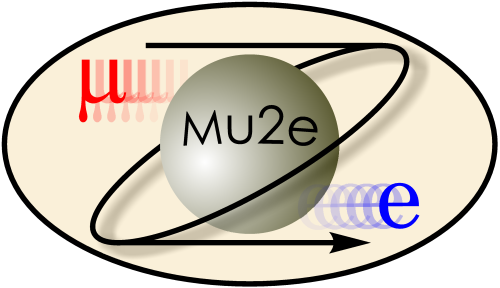
\includegraphics[width=0.5\textwidth]{mu2e_logo_oval.png}\par\vspace{2cm}
	{\scshape\LARGE CO$_2$ Leak Testing of Straws \\
		Standard Operating Procedure \\ Version 3.0 \par}
	\vspace{3cm}
	{\Large Sam Penders\par}
    \vspace{.5cm}
	\vspace{3cm}
	{\large University of Minnesota\par}
 	\vspace{.5cm}
	{\large June 7, 2018\par}
	% Bottom of the page
	\vfill
	{\href{mailto:pende061@physics.umn.edu}
    {\tt{pende061@physics.umn.edu}}\par}
	
    {\href{Linds551@umn.edu}
    {\tt{Linds551@umn.edu}}\par}
\end{titlepage}

\clearpage
\setcounter{page}{1}

\newenvironment{myitemize} %adjust item spacing in lists to make smaller
{ \begin{itemize}
    \setlength{\itemsep}{4pt}
    \setlength{\parskip}{0pt}
    \setlength{\parsep}{0pt}     }
{ \end{itemize}                  } 

\section{Goal}
All Mylar straws in the Mu2e electron tracker panels will be inflated with a mix of argon gas and CO$_2$ during the run of the experiment. Thus, our goal is to determine the leak rate of each straw before panel installation, as well as identify straws that are damaged. We strive to do this in a safe, efficient, and reproducible manner.

%-----------------------------------------------
%	EQUIPMENT
%-----------------------------------------------

\section{Equipment Used}
\begin{multicols}{2}
\begin{myitemize}
	\item Pallet with Mylar straws
	\item An empty pallet
	\item CO$_2$ tank with regulator attached
	\item N$_2$ tank with regulator attached
	\item CO$_2$ pressure gauge and flow meter with hose 
	\item Vacuum grease
	\item Straw end-piece hose plugs
	\item Leak test chambers
	\item Plastic straw loading tubes
	\item Magnetic grabber
	\item Arduino Unos connected to leak chambers and computer
	%\item Isopropyl alcohol and paper towels
	\item Form--fitting nitrile gloves
\end{myitemize}
\end{multicols}

%-----------------------------------------------
%	RISKS AND DANGERS
%-----------------------------------------------

\section{Risks and Dangers}
There is an inherent danger when working with pressurized gases. Because the N$_2$ and CO$_2$ tanks are pressurized to a maximum of 2500 psi, an uncontrolled discharge of gas from the cylinders would effectively make the cylinders into rockets. This could happen if a cylinder is knocked over and the gas cylinder valve or regulator valve gets damaged. For this reason, compressed gas chambers are harnessed to the wall by a chain. The regulator over the exit valve limits the pressure of gas released from the chamber. To prevent accidental tipping of the cylinders, only a trained supervisor should ever move cylinders or adjust regulator pressure. 

High levels of CO$_2$ in the air can make a person feel dizzy. To CO$_2$ levels from getting high, the lab has a good ventilation system. Make sure that you can hear the sound of fans from the laboratory ventilation system when working with the CO$_2$. If you do feel dizzy, close the CO$_2$ tank valve and step outside for a few minutes. Always close the gas tanks when not in use.

%Care must be taken when cleaning with isopropyl alcohol. Contact with skin can cause irritation, so nitrile gloves should be worn at all times. If alcohol gets on skin, it should be washed off with soap and water. If alcohol gets in your eyes, they should be rinsed in the eye wash for several minutes. Then, go to a doctor.


\newpage

\section{Leak Testing Procedure}

\subsection{Setup}
\begin{enumerate}
	\item Put on nitrile gloves that fit snuggly. These must be worn at all times when handling straws.
	\item Check that the regulator is attached to CO$_2$ tank. Do not touch center regulator knob. Open both the gas cylinder and regulator exit valve completely. (Figure \ref{co2tank}) If these are only partially opened, gas may leak from the valve.   
	\item Check cylinder pressure. If below 200 psi, stop using cylinder immediately. If below 500 psi, have Dan order a new cylinder.
	\item Adjust flow gauge (Figure \ref{flow gauge}) on near pressure gauge to 10 scfh. Cover end of CO$_2$ nozzle with finger and confirm that the pressure on near pressure gauge reads $15.0 \pm 0.1$ psi. If not, consult a supervisor.
\end{enumerate}

\begin{figure}
	\centering
	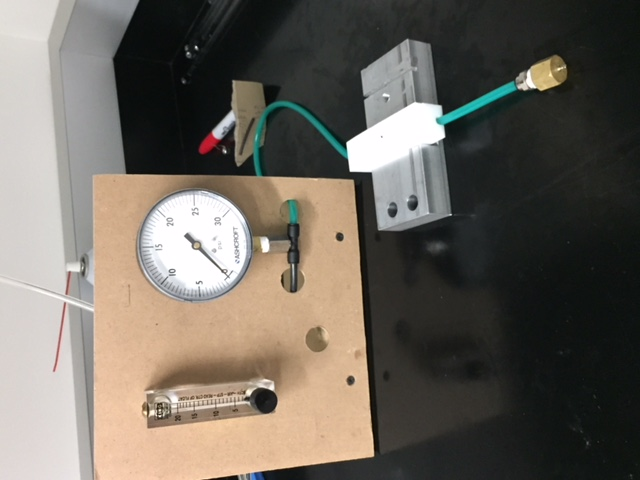
\includegraphics[width=0.6\textwidth,angle=-90]{flow_gauge}
	\caption{Flow gauge. The left gauge adjusts the flow rate, and should be set to 10 scfh. The right gauge shows the gas pressure, which should be approximately 15 PSI.}
	\label{flow gauge}
\end{figure}

\begin{figure}
	\center
	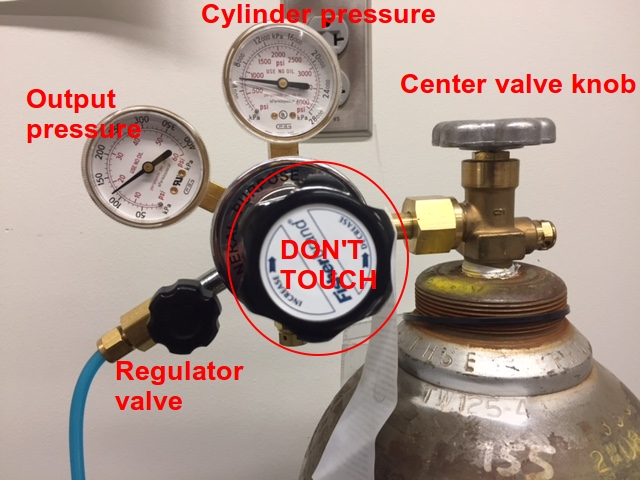
\includegraphics[scale=0.5]{co2tank}
	\caption{CO$_2$ tank with regulator attached. The regulator adjustment knob in the center should not be adjusted. The N$_2$ tank regulator is identical.} \label{co2tank}
\end{figure}


\subsection{Inflating Straws} \label{performing test}
{\bf Note: Avoid bending the straws in any way}
	\begin{enumerate}
		\item Gently hold an endpiece hose with the pliers, resting the plier's tip on the pallet. With the CO$_2$ on and the flow gauge set to 10 scfh, insert the nozzle on the CO$_2$ hose into the first straw endpiece hose. \label{flush step}
		\item While the CO$_2$ flushes the straw, apply a minimal amount of vacuum grease to a hose plug. Hold the endpiece hose on the side opposite with the pliers, as in step \ref{flush step}, and insert the plug. The straw should have flushed for $\sim 10$ seconds.
		\item Apply a minimal amount of vacuum grease to another endpiece plug. On the CO$_2$ hose side of straw, pinch the end-piece hose with pliers while resting the pliers firmly against the pallet, and pull the CO$_2$ hose away from the hose. While continuing to pinch the hose, insert the plug into the straw hose.
		\item Listen for a leak in the straw. If you hear one, try to find where it is coming from and circle the hole. Do not bother leak testing a straw with an apparent leak.
		\item Repeat for all straws on the pallet.
		\item With a cotton swab, wipe off all excess vacuum grease from the endpiece hoses.

\subsection{Loading and Flushing Chambers}	
		\item Transfer the pallet full of straws to the table by the leak testing chambers. Place the empty pallet with its end next to the end of the full one and place 24 plastic loading tubes onto the empty pallet (Figure \ref{tubes on pallet}).	Note that the ends of the tubes with nuts on them are away from the straws.	
		\item Carefully lift the end of a straw about by the hose about 1 cm. Slide a plastic tube onto the straw to about half of the straw's length. Lift up the other end of the straw by the hose, and slide the rest of the straw into the tube. Repeat for all straws.
		 \item Pick up a tube with a straw inside and slide it into a leak chamber, with the end of the tube with the nut going in last. Leave the end of the chamber open, and turn the black nitrogen valve clockwise on the leak chamber to allow nitrogen to flush out the chamber. \label{load}
		 \item Go get another loading tube with a straw inside, and put it into the next chamber, in the same way as Step \ref{load}. Now, close the nitrogen valve on the previous chamber, and close the loading valve on the previous chamber. {\bf Close the nitrogen valve, THEN close the loading valve. The previous chamber should have flushed for about 15 seconds.} With the loading valve open on the chamber you just filled, open its nitrogen value (clockwise). Repeat this step until all straws are in a chamber.
		 \item When all chambers are loaded and flushed, close the two valves on the nitrogen tank.
		 
\begin{figure}
	\centering
	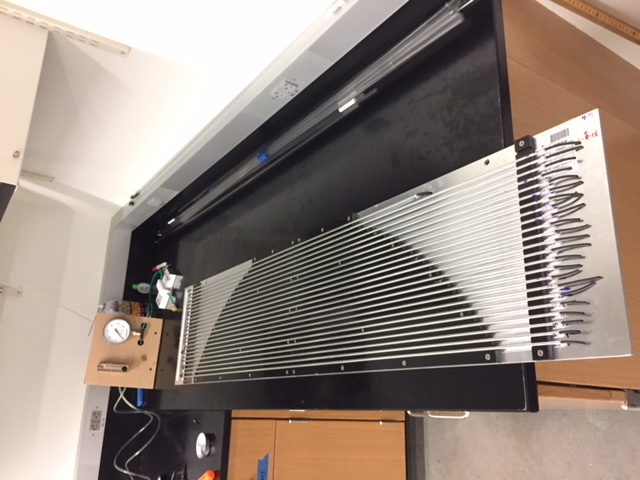
\includegraphics[width=0.6\textwidth, angle=-90]{inflate_setup}
	\caption{Straw inflation setup.}
	\label{inflate setup}
\end{figure}
        
\end{enumerate}

\begin{figure}
	\centering
	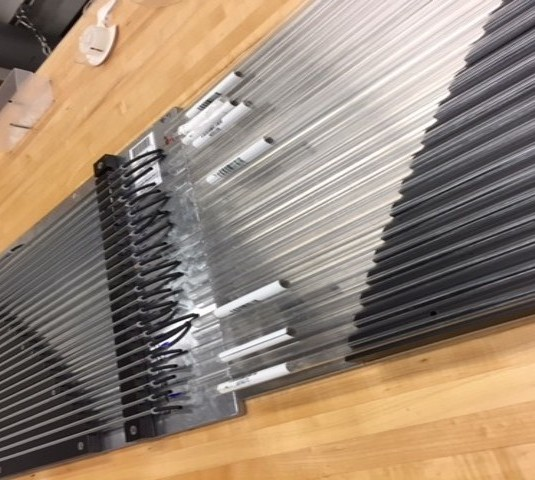
\includegraphics[width=0.5\textwidth,angle=-90]{adjacent_pallets}
	\caption{Two pallets aligned to slide plastic tubes onto inflated straws.}
	\label{tubes on pallet}
\end{figure}


\subsection{Measuring Leak Rate}
	\begin{enumerate}
    	\item Open the leak test GUI, named {\tt Leak Test GUI Launcher.py}, located on the desktop.  A picture of the right-half of the GUI is shown in figure \ref{GUI}.
        \item Click the login button on the top of the GUI screen and enter your name.
        \item Make sure all nitrogen valves on the leak chambers are closed, and all leak test chambers are closed.
        \item To start taking data on a specific row, click the "Start Data" button below the desired chamber row.  When a chamber row is active the square in which the number resides will turn green.
        \item To load each straw, click ``Load Straw'', scan the straw barcode into the box, and click ``OK.'' This is quickest if one person clicks on the boxes, and one person scans the barcodes.
        \item Straws take 45-60 minutes to test.  A plot of the measured data can be viewed for each straw by clicking the ``Plot'' icon below each straw. This can be used to make sure straw leak rates are being measured correctly. A good straw will have a clearly linear leak plot.
        \end{enumerate}

\begin{figure}[ht]
	\center
	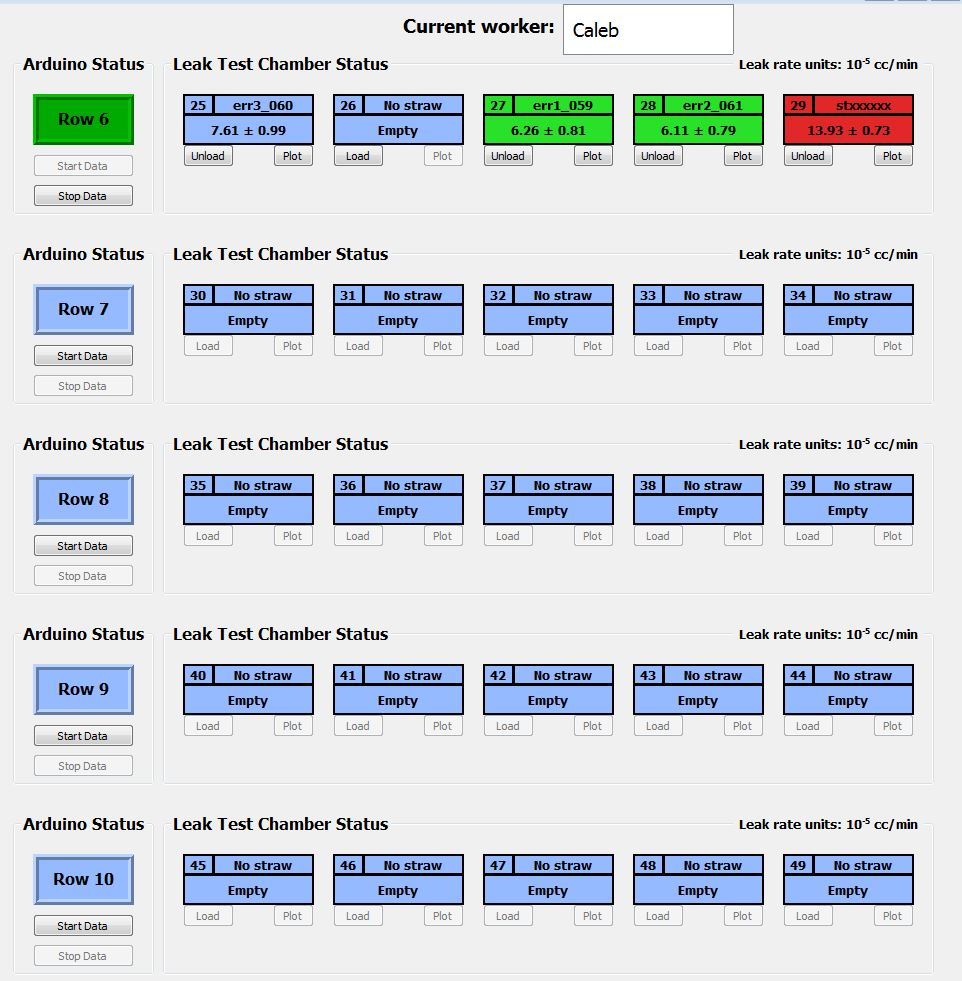
\includegraphics[scale=0.5]{GUI}
	\caption{Right-half of the Leak Test GUI.  Row 6 is the only row running.  The straws with green backgrounds pass, the red one has failed, and the blue ones are either empty or still testing.} \label{GUI}
\end{figure}






\subsection{Emptying Leak Chamber}
	\begin{enumerate}
		\item When a straw is done testing it will light up either red or green.  Green straws meet the minimum leak rate requirement, but red ones have failed.  
	\item Before physically removing finished straws, click ``Unload'', and make sure the straw name disappears from the GUI.  
	\item Open the white lever and use the magnetic grabber to gently remove the tube. Place the tube on the pallet spot the straw came from, and carefully slide the tube off of the straw so the straw goes back in its place. Carefully pull the plugs out of the straw hoses and put them back into their bin.
	\item Repeat for all straws.
	\item If a row has no straws being tested, click "Stop Data" to turn it off.
	\item Put a check mark in the box next to the straw in the ``L'' section (``L'' for ``leak'') if the straw passed. If it failed, but a ``X in the box.
	''
\end{enumerate}

\subsection{Cleanup}
	\begin{enumerate}
		\item Make sure that N$_2$ and CO$_2$ cylinder and regulator valves are closed.
		\item Put any extra straw end-piece hose plugs back into their container.
		\item Wipe and clean any vacuum grease off of work surface with alcohol and paper towel.
		\item Throw away gloves|they likely have vacuum grease on them.
	\end{enumerate}



\section{Troubleshooting}

\begin{itemize}
	\item {\bf Problem:} One of the chambers isn't taking data.
		\begin{adjustwidth}{1cm}{}
		{\bf Solution:} Make sure that the sensor cable is attached to the chamber, and is plugged securely into its Arduino port. If this doesn't work, sometimes the CO$_2$ level offset can be initially to low in the chamber. Open the straw loading valve and exhale for about half a second into chamber, then close valve. If this does not help, unplug Arduino from power supply for a minute. Then replug and try again. If the problem persists, ask for help.
		\end{adjustwidth}
\item {\bf Problem:} A straw is stuck in the chamber.
		\begin{adjustwidth}{1cm}{}
		{\bf Solution:} Unplug sensor cable from chamber, and slide entire chamber off of rack. With the straw loading valve open and hold over valve, tip chamber upside down and try to shake straw out. If this doesn't work, try to grab onto the straw with claw grabber. If this doesn't work, consult manager.
		\end{adjustwidth}
        \item {\bf Problem:} Starting a row causes the GUI to crash
		\begin{adjustwidth}{1cm}{}
		{\bf Solution:} Likely an arduino error.  Make sure the sensor cable is securely connected to the arduino port.  If it is, unplug the arduino for 30 seconds and plug it back in.
		\end{adjustwidth}
        \item {\bf Problem:} The straw I entered disappeared from the GUI
		\begin{adjustwidth}{1cm}{}
		{\bf Solution:} The program is likely still collecting data, but the straw information is not showing up.  Click "Load" and enter the straw ID again.  The straw information should return right away.  If not, ask a manager for help.
		\end{adjustwidth}
	\item {\bf Problem:} I accidentally entered the wrong straw for a chamber.
		\begin{adjustwidth}{1cm}{}
		{\bf Solution:} Empty the chamber in the program. Ask a manager to delete the incorrectly named file. Re-enter the correct straw in the leak test program.
		\end{adjustwidth}
\item {\bf Problem:} A straw is epoxied at the end-piece to the pallet, so I can't remove it.
		\begin{adjustwidth}{1cm}{}
		{\bf Solution:} Carefully try to peel stuck end off of plastic. If it looks okay, leak test it as usual. If it is obviously damaged, cut damaged end off of straw and give to epoxy station to re-epoxy an endpiece in.
		\end{adjustwidth}
		

\end{itemize}











\end{document}
